%   =============================
%		Change document settings here 
%   =============================

% TITLEPAGE SETTINGS
% ------------------
\newcommand{\docAutor}				{various}								% name of the author of the book
\newcommand{\docTitel}				{Algorithms I}			% title of the lecture/book
\newcommand{\docUntertitel}			{Lecture Notes of Spring 2013}		% subtitle
\newcommand{\docDozent}				{tbd}			% name of the professor
\newcommand{\docJahr}				{2013}			% publishing year
\newcommand{\docUniversitaet}	{University of Mannheim}	% name of university
\newcommand{\docTitelZitat}		{}
\newcommand{\docTitelZitatName}	{}				% titlepage quote author

% GENERAL SETTINGS
% ----------------
\newcommand{\useIndex}					{0} 											% set '1' if you want to include an index
\newcommand{\useThumbs}					{0}												% set '1' if you want to use chapter thumbs on the page side
\newcommand{\useRoman}					{0}												% set '1' if you want to have chapter numbering with roman numbers

\newcommand{\usrBCOR}					{0cm}    										% set binding correction offset here (space lost on the inner borders due to binding)
\newcommand{\usrmatter}					{0}												% set '1' to start numbering at actual content beginning
\newcommand{\usroptsqrt}				{1}												% set '1' to use alternate form for roots with a small closing line
\newcommand{\usrnscmd}[1]				{\textbf{#1}}							% set e.g. '\textbf', '\mathbb' or '\mathds' for namespace macros
				% document specific settings

\documentclass[a4paper, 						% paper size
							 12pt, 								% font size
							 BCOR = \usrBCOR,			% binding correction
							 DIV=15, 							% used for typearea calculation
							 headsepline,					% add head line to border calculation
							 footnotes = multiple,% visually separate two consecutive footnotes
							 toc = index,					% add index to table of contents
							 numbers = auto,			% automatic placing of end dot in numbering\deftxt{Hamiltonian}\deftxt{Hamiltonian}
							 pagesize							% used for flexibility
							]{scrreprt}
							
% PREAMBLE
% =========
					
\usepackage[english]{babel}
\usepackage[latin1]{inputenc}					% input encoding
\usepackage[T1]{fontenc}							% use T1 fonts for font encoding
\usepackage{amsfonts}									% math font
\usepackage{newcent}									% use New Century Schoolbook
\usepackage{fouriernc}								% math font for newcent
\usepackage{dsfont}										% math font for number spaces etc.
\usepackage{helvet}										% sans serif font
\usepackage{inconsolata}							% font for typewriter style

% general
\usepackage{makeidx}
\makeindex

\usepackage{ifthen}
\usepackage{letltxmacro}							% better support for redefining macros with optional arguments
\usepackage{booktabs}									% nicer tables
\usepackage{wrapfig}									% text around figures
\usepackage{parskip}									% vertical space instead of indentation
\usepackage{microtype}								% improved justification
\usepackage{needspace}								% reserve space
\usepackage{framed}										% shaded environments
\setlength{\FrameSep}{0pt}						% correct colorbox width (package: framed)

\usepackage{xcolor}
\usepackage{graphicx}
\usepackage{tikz}
\usetikzlibrary{positioning}
\usetikzlibrary{arrows}

\usepackage{enumitem}
\setenumerate[1]{label=\roman*)}			% roman numbered lists
\setitemize			{leftmargin=*}
\setenumerate		{leftmargin=*}


\usepackage{chapterthumb}							% use chapter thumbs
\setkomafont{chapterthumb}						% use small font for chapter thumbs
	{\normalfont\sffamily}
\renewcommand{\chapterthumbheight}		% make chapter thumbs thinner
	{1em}
	
\setkomafont{chapterentry}						% no sans-serif but bold chapter entries in toc
	{\normalfont\bfseries}
\setkomafont{chapterentrypagenumber}	% no bold chapter page entry numbers in toc
	{\normalfont}
	
\renewcommand{\footnoterule}{					% increase spacing below footnote line
	\noindent\rule{0.4\textwidth}{.4pt}
	\vspace{0.6em}}
\deffootnote{1em}{1em}								% footnote in normal textsize
	{\thefootnotemark\hspace{0.5em}}
	
\usepackage{scrpage2}
\setkomafont{pageheadfoot}
	{\normalfont\itshape}
\pagestyle{scrheadings}								% switch to modified style

\renewcommand{\chaptermark}[1]
	{\markboth{\thechapter~#1~}{}}
\renewcommand{\sectionmark}[1]
	{\markright{\thesection\autodot~#1}}
					
\usepackage{titlesec}									% design chapter headings
\titleformat{\chapter}[display]
	{\normalfont\sffamily\Huge\bfseries\flushright\fontsize{70}{0}\selectfont}
	{\thechapter}
	{-0pt}{\Huge}
\setkomafont{section}{\normalfont\Large\bfseries}
\setkomafont{subsection}{\normalfont\large\bfseries}
\titlespacing*{\chapter}{0pt}{0pt}{50pt}

\ifthenelse{\equal{\useRoman}{1}}									% roman chapter numbering
	{\renewcommand{\thechapter}{\Roman{chapter}}}{}
					
\clubpenalty 					= 10000					%
\widowpenalty 				= 10000					% avoid widow and club lines
\displaywidowpenalty 	= 10000					%

\makeatletter
\@beginparpenalty			=	10000					% avoid page breaks before lists
\makeatother

\definecolor{linkblue}{rgb}{0.0, 0.0, 0.3}
\definecolor{citeblue}{rgb}{0.0, 0.0, 0.5}
\usepackage[pdfstartpage				= 1,							% default opening start page 
						pdfstartview				= FitB, 					% default opening zoom
						pdftitle						= {\docTitel},		% document title
						pdfauthor						= {\docAutor}, 		% document author
						colorlinks					= true, 					% print links colored
						bookmarks						= true, 					% use bookmarks
						bookmarksopen				= true,						% open bookmarks by default
						bookmarksnumbered		= true, 					% number bookmarks
						linkcolor						= linkblue,					% color for links
						citecolor						= citeblue,				% color for cite links
						pdfdisplaydoctitle	= true						% display document title instead of file name
					 ]{hyperref}

% mathematical
\usepackage{amssymb}
\usepackage{amsmath}
\usepackage{amsthm}
\usepackage{latexsym}
\usepackage{stmaryrd}
\usepackage{esint}										% provides \ointclockwise etc.
\usepackage{mathtools}								% provides \xRightarrow[]{}, \mathclap, \shortintertext and \bigtimes

\makeatletter																			% alternate closed root symbol
\ifthenelse{\equal{\usroptsqrt}{1}}{%
\let\oldr@@t\r@@t
\def\r@@t#1#2{%
\setbox0=\hbox{$\oldr@@t#1{#2\,}$}\dimen0=\ht0
\advance\dimen0-0.2\ht0
\setbox2=\hbox{\vrule height\ht0 depth -\dimen0}%
{\box0\lower0.65pt\box2}}
\LetLtxMacro{\oldsqrt}{\sqrt}
\renewcommand*{\sqrt}[2][\ ]{\oldsqrt[#1]{#2}}}{}
\makeatother				% general settings and packages
\newcommand{\A}{\usrnscmd A}
\newcommand{\B}{\usrnscmd B}
\newcommand{\C}{\usrnscmd C}
\newcommand{\D}{\usrnscmd D}
\newcommand{\E}{\usrnscmd E}
\newcommand{\F}{\usrnscmd F}
\newcommand{\G}{\usrnscmd G}
%\renewcommand{\H}{\usrnscmd H}						% only activate if needed
\newcommand{\I}{\usrnscmd I}
\newcommand{\J}{\usrnscmd J}
\newcommand{\K}{\usrnscmd K}
%\renewcommand{\L}{\usrnscmd L}						% only activate if needed
\newcommand{\M}{\usrnscmd M}
\newcommand{\N}{\usrnscmd N}
%\renewcommand{\O}{\usrnscmd O}						% only activate if needed
%\renewcommand{\P}{\usrnscmd P}						% only activate if needed
\newcommand{\Q}{\usrnscmd Q}
\newcommand{\R}{\usrnscmd R}
\renewcommand{\S}{\usrnscmd S}
\newcommand{\T}{\usrnscmd T}
\newcommand{\U}{\usrnscmd U}
\newcommand{\V}{\usrnscmd V}
\newcommand{\W}{\usrnscmd W}
\newcommand{\X}{\usrnscmd X}
\newcommand{\Y}{\usrnscmd Y}
\newcommand{\Z}{\usrnscmd Z}

\newcommand{\sA}{\mathcal A}
\newcommand{\sB}{\mathcal B}
\newcommand{\sC}{\mathcal C}
\newcommand{\sD}{\mathcal D}
\newcommand{\sE}{\mathcal E}
\newcommand{\sF}{\mathcal F}
\newcommand{\sG}{\mathcal G}
\newcommand{\sH}{\mathcal H}
\newcommand{\sI}{\mathcal I}
\newcommand{\sJ}{\mathcal J}
\newcommand{\sK}{\mathcal K}
\newcommand{\sL}{\mathcal L}
\newcommand{\sM}{\mathcal M}
\newcommand{\sN}{\mathcal N}
\newcommand{\sO}{\mathcal O}
\newcommand{\sP}{\mathcal P}
\newcommand{\sQ}{\mathcal Q}
\newcommand{\sR}{\mathcal R}
\newcommand{\sS}{\mathcal S}
\newcommand{\sT}{\mathcal T}
\newcommand{\sU}{\mathcal U}
\newcommand{\sV}{\mathcal V}
\newcommand{\sW}{\mathcal W}
\newcommand{\sX}{\mathcal X}
\newcommand{\sY}{\mathcal Y}
\newcommand{\sZ}{\mathcal Z}

\newcommand{\deftxt}[1]											% emphasize newly defined terms
	{\textcolor{def_color}{#1}}

\renewcommand{\I}{\mathrm i}								% imaginary unit
\newcommand{\dd}{\mathrm d}									% differential
\newcommand{\e}{\varepsilon}								% nicer epsilon
\newcommand{\id}{\operatorname{id}}					% identity operator
\newcommand{\ind}{\textbf{1}}								% indicator function
\newcommand{\norm}[1]{\left\|#1\right\|}		% norm
\renewcommand{\Re}{\operatorname{Re}}				% real part
\renewcommand{\Im}{\operatorname{Im}}				% imaginary part

% statistic-related
\newcommand{\Pois}{\operatorname{Pois}}			% Poisson distribution
\newcommand{\Var}{\operatorname{Var}} 			% variance
\newcommand{\Cov}{\operatorname{Cov}}				% covariance
\newcommand{\Binom}{\operatorname{B}}				% binomial distribution
\newcommand{\Bias}{\operatorname{Bias}}	% predefined macros
\definecolor{def_color}					{HTML}{194D6C}
\definecolor{def_shade_color}		{HTML}{DFE9EF}
\definecolor{thm_color}					{HTML}{2F2512}
\definecolor{thm_shade_color}		{HTML}{FFF7D4}	

\newlength{\internalindent}
\setlength{\internalindent}		% defines how much text and lists are intended
	{.5cm}
	
\newtheoremstyle{thmstyle}
	{\internalindent}
	{\internalindent}{
		\addtolength{\leftskip}	{\internalindent}					 
		\addtolength{\rightskip}{\internalindent}
	}
	{0pt}{}{}
	{\newline}
	{\textcolor{thm_color}{\textbf{#1} #2} \quad  \textbf{#3}}
	
\newtheoremstyle{defstyle}
	{\internalindent}
	{\internalindent}{
		\addtolength{\leftskip}	{\internalindent}					 
		\addtolength{\rightskip}{\internalindent}
	}
	{0pt}{}{}
	{\newline}
	{\textcolor{def_color}{\textbf{#1} #2} \quad  \textbf{#3}}
	
\newtheoremstyle{bspstyle}
	{\internalindent}
	{\internalindent}{
		\addtolength{\leftskip}	{0pt}					 
		\addtolength{\rightskip}{0pt}
	}
	{0pt}{}{}
	{\newline}
	{\textbf{#1} #2 \quad  \textit{#3}}
	
\theoremstyle{thmstyle}
\newtheorem{tmp_satz}{Theorem}[chapter]
\newtheorem{tmp_kor}{Korollar}[chapter]
\newtheorem{tmp_lemma}{Lemma}[chapter]
\newtheorem{tmp_prop}{Proposition}[chapter]

\theoremstyle{defstyle}
\newtheorem{tmp_def}{Definition}[chapter]

\theoremstyle{bspstyle}
\newtheorem{tmp_bsp}{Example}[chapter]
\newtheorem*{tmp_bsp*}{Example}

\newenvironment{theorem}[1][]{
	\setlist			{rightmargin=\internalindent}
	\setitemize		{leftmargin=\leftmargin}
	\setenumerate	{leftmargin=\leftmargin+\internalindent}
	\definecolor{shadecolor}{named}{thm_shade_color}
	\needspace{4\baselineskip}
	\begin{shaded}\begin{tmp_satz}[#1]
}{
	\end{tmp_satz}
	\end{shaded}
	\noindent\ignorespacesafterend
}
	
\newenvironment{korollar}[1][]{
	\setlist			{rightmargin=\internalindent}
	\setitemize		{leftmargin=\leftmargin}
	\setenumerate	{leftmargin=\leftmargin+\internalindent}
	\definecolor{shadecolor}{named}{thm_shade_color}
	\needspace{4\baselineskip}
	\begin{shaded}\begin{tmp_kor}[#1]
}{
	\end{tmp_kor}
	\end{shaded}
	\noindent\ignorespacesafterend
}

\newenvironment{lemma}[1][]{
	\setlist			{rightmargin=\internalindent}
	\setitemize		{leftmargin=\leftmargin}
	\setenumerate	{leftmargin=\leftmargin+\internalindent}
	\definecolor{shadecolor}{named}{thm_shade_color}	
	\needspace{4\baselineskip}
	\begin{shaded}\begin{tmp_lemma}[#1]
}{
	\end{tmp_lemma}
	\end{shaded}
	\noindent\ignorespacesafterend
}
	
\newenvironment{proposition}[1][]{
	\setlist			{rightmargin=\internalindent}
	\setitemize		{leftmargin=\leftmargin}
	\setenumerate	{leftmargin=\leftmargin+\internalindent}
	\definecolor{shadecolor}{named}{thm_shade_color}
	\needspace{4\baselineskip}
	\begin{shaded}\begin{tmp_prop}[#1]
}{
	\end{tmp_prop}
	\end{shaded}
	\noindent\ignorespacesafterend
}
	
\newenvironment{definition}[1][]{	
	\setlist			{rightmargin=\internalindent}
	\setitemize		{leftmargin=\leftmargin}
	\setenumerate	{leftmargin=\leftmargin+\internalindent}
	\definecolor{shadecolor}{named}{def_shade_color}
	\needspace{4\baselineskip}
	\begin{shaded}\begin{tmp_def}[#1]
}{
	\end{tmp_def}
	\end{shaded}
	\noindent\ignorespacesafterend
}

\DeclareRobustCommand{\bspendmark}{% defines end mark for examples
	\ifmmode \quad\sslash
	\else	\hbox{$\sslash$}
	\fi
}

\newenvironment{example}[1][]{	
	\pushQED{\bspendmark}
	\needspace{4\baselineskip}
	\begin{tmp_bsp}[#1]
}{
	\end{tmp_bsp}
	\noindent\ignorespacesafterend
}

\newenvironment{example*}[1][]{	
	\pushQED{\bspendmark}
	\needspace{4\baselineskip}
	\begin{tmp_bsp*}[#1]
}{
	\end{tmp_bsp*}
	\noindent\ignorespacesafterend
}
	
\renewcommand*\proofname{Proof}
\makeatletter
\newenvironment{prooof}[1][\proofname]{
	\par
	\normalfont \topsep6\p@\@plus6\p@\relax
	\trivlist
	\item[\hskip\labelsep
		\bfseries #1\@addpunct{:}]~%\newline\ignorespaces
}{
	\endtrivlist\@endpefalse
	\noindent\ignorespacesafterend
}
\makeatother

\newsavebox{\informationbox}
\newenvironment{information}
{\begin{center}\begin{lrbox}{\informationbox}\begin{minipage}{0.7\textwidth}\small}
{\end{minipage}\end{lrbox}
\begin{tikzpicture}

\draw[fill] (-0.5*\wd\informationbox - 1cm, 0.1cm) circle (0.3cm);
\draw[color=white] (-0.5*\wd\informationbox - 1cm, 0.1cm) node {\large\bfseries i};

\draw (0,0) node {\usebox{\informationbox}};
\end{tikzpicture}\end{center}
}

\newcommand{\boffset}{7pt}			% space the frame surrounds the text
\newcommand{\bthickness}{1pt}
\newcommand{\blength}{4*\bthickness}
\newsavebox{\chapdescbox}
\newenvironment{descr}
{\begin{center}\begin{lrbox}{\chapdescbox}\begin{minipage}{0.9\textwidth}}
{\end{minipage}\end{lrbox}
\begin{tikzpicture}
	\draw[fill] (-0.5*\wd\chapdescbox - \boffset - \bthickness, \ht\chapdescbox + \boffset + \bthickness) 	rectangle
							(-0.5*\wd\chapdescbox - \boffset							, \ht\chapdescbox + \boffset - \blength);
	\draw[fill]	(-0.5*\wd\chapdescbox - \boffset - \bthickness, \ht\chapdescbox + \boffset + \bthickness) 	rectangle
							(-0.5*\wd\chapdescbox - \boffset + \blength		, \ht\chapdescbox + \boffset);
							
	\draw[fill]	(0.5*\wd\chapdescbox + \boffset								, -\dp\chapdescbox - \boffset - \bthickness) 	rectangle
							(0.5*\wd\chapdescbox + \boffset + \bthickness	, -\dp\chapdescbox - \boffset + \blength);
	\draw[fill]	(0.5*\wd\chapdescbox + \boffset + \bthickness	, -\dp\chapdescbox - \boffset) 								rectangle
							(0.5*\wd\chapdescbox + \boffset - \blength		, -\dp\chapdescbox - \boffset - \bthickness);
	
	\draw (0,0) node {\usebox{\chapdescbox}};
\end{tikzpicture}\end{center}
}
		% predefined environments
%
% define how to hyphenate certain words in case you're experiencing problems with them
% use the following command pattern:
% \hyphenation{hy-phe-na-te}
%
		% custom hyphenation rules

%\includeonly{}											% while writing your book, compile only what you need

\begin{document}
\raggedbottom
\ifthenelse{\equal{\usrmatter}{1}}
	{\frontmatter}{}
\begin{titlepage}
\raggedleft
{\large \docAutor\\[1in]}
{\large \docUntertitel\\[.2in]}
{\fontsize{35}{0}\selectfont\bfseries\docTitel\\[.2in]}
\ifthenelse{\equal{\docTitelZitat}{}}{}
{{\footnotesize{\itshape \docTitelZitat}\\\docTitelZitatName\\}}
\vfill
{\large \docUniversitaet\\\docJahr}
\end{titlepage}

\newpage
\thispagestyle{empty}

\markboth{Legal Notes}{Legal Notes}

\noindent This script originates from the course "`\docTitel"' at the University of Mannheim as lecture notes.

The accuracy of its content is not guaranteed and the author(s) do not assume responsibilitty for possible damages of any kind.
This lecture notes are not an official document released by employees of the University of Mannheim, hence those do not assume responsibility, as well.

Many thanks to Ingo B�rk, who initially published the underlying LaTeX template \href{http://www.matheboard.de/thread.php?threadid=498961}{here}.
This work is licensed under a \href{http://creativecommons.org/licenses/by-nc-sa/3.0/de/deed.en_US}{Creative Commons Attribution-NonCommercial-ShareAlike 3.0 Germany License}.
\newpage
\tableofcontents
\ifthenelse{\equal{\usrmatter}{1}}
	{\mainmatter}{}
\ifthenelse{\equal{\useThumbs}{1}}
	{\ihead[\putchapterthumb]{\putchapterthumb}}{}
	
% ================================
% include your document parts here
% only use section-wise documents since include inserts new pages!
\chapter{TODO: Elementary Notions about Graphs}

\begin{descr}
    TODO
\end{descr}


\begin{definition}
	An undirected graph is a pair G=(V, E) where V is a set of nodes and E is a set of edges, together with a function i: E $\rightarrow \gamma(v)$ such that 0 < $\mid i(e) \mid  \le $ 2.
\\
If u,v i(e) we call u,v endpoints of e. If V and E are a finite set we call G a finite graph. If i($e{_1}$) =  i($e{_2}$) we call  $e{_1}$, $e{_2}$ parallel edges.

If $\mid i(e) \mid = 1$ we call e a loop. The degree of a node v is the number of edges for which v is an endpoint where loops a counted twice.
Is the degree of v = 0 then we call v isolated.
\end{definition}

\begin{example*}
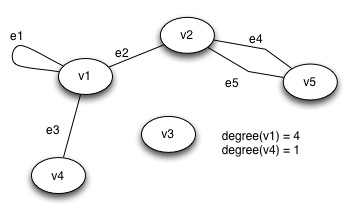
\includegraphics{diagrams/Chapter1_Example1.jpg} \\
\end{example*}

\begin{lemma}
    In a finite graph the number of nodes with odd degree is even.
\end{lemma}


\begin{prooof}
    $\sum\limits_{i=1}^n degree(v{_i}) = 2* \mid E \mid$ \\
This is because we start with a graph, where each node is isolated. Then we insert one edge after another.\\
Case 1: i(e) = {x} then the degree of x is increased by 2\\
Case 2: i(e) = {x, y} then the degree of x and y are increased by 1\\
We asume that $v{_1}...v{_i}$ have an even degree and $v{_i+1}...v{_n}$ have odd degree.\\

$\sum\limits_{k=1}^i degree(v{_k}) + \sum\limits_{k=i+1}^n degree(v{_k}) = 2 \mid E \mid$\\

$\sum\limits_{k=1}^i degree(v{_k})$ is an even number\\

$\sum\limits_{k=i+1}^n degree(v{_k})$ must be an even number and hence the number of nodes with odd degree must be even\\

$ 2 \mid E \mid$ is an even number \\

\end{prooof}


\begin{definition}
    If G=(V,E) is a graph and $v{_1}, v{_2} \in V$ with $i(e) = \{v1, v2\}$ then we say that $v{_1}, v{_2}$ are neighbours. A path in G is a sequence of edges $e{_1}, e{_2}, ...$ such that: \\
\begin{enumerate}
\item $e{_i}, e{_i+1}$ share an endpoint
\item if $e{_i}$ is not a loop and neither the first nor the last edge. Then $e{_i}$ shares one endpoint with $e{_i-1}$ and the other with $e{_i+1}$ [MS: does this make sense? sounds strange!]
\end{enumerate}
\end{definition}

\begin{example*}
TODO: Graphic missing\\
\end{example*}

A finite graph is graphically represented by: $v{_0}$ --- $v{_1}$ --- $v{_2}$ --- ... --- $v{_i}$\\
$v{_0}$ is called start point and $v{_i}$ is called end point. The length of the path $e{_1}$ ... $e{_i}$  is $i$.\\
\\
A cycle (circle) is a path where the end point coincide with the start point.\\
A path is called simple if every node in $V$ occures at most once.\\
A cycle of length $\not = 2$ is called simple if every node except of the start/end node occurs at most once. A cycle of length 2 ($e{_1}$, $e{_2}$) is called simple if $e{_1} /not = e{_2}$ and if each node except for the start/end node occurs at most once.

\begin{example*}
TODO: Graphic missing\\
\end{example*}

A Graph is connected if for every pair of nodes ($u$, $v$) there is a path between $u$ and $v$.\\

An infinite Graph has finite and infinite paths. Every path between two nodes is finite. The graph is connected. There are infinitely paths.\\
e.G. $e{_1}$ (finite)\\
or $e{_1}$, $e{_2}$\\
...\\
and there is also an infite path $e{_1}$, $e{_2}$, $e{_2}$, $e{_2}$, $e{_2}$, $e{_2}$, ...\\


\begin{definition}
    Let $G(V,E)$ be a connected graph $a \in V$ is called a seperation point (articulation point) if there are nodes $v, w$ such that every path connecting $v$ and $w$ visits $a$. If $G$ has such a point $G$ is called [word missing - MS]\\
    An edge is called bridge if there exist nodes $v$, $w$ such that every path connecting $v$ and $w$ contains this edge.
\end{definition}

\begin{example*}
Real-Life examples where seperation points are important are in computer networks or the information distribution (flow of information) within a company. So a seperation point can be regarded as a kind of coordinator between $a$ and $b$.
\end{example*}

\begin{definition}
    Let $G = (V,E)$ be a graph without loops. If there exists $V_{1}, V_{2} \leq V$ and $V_{1} \cup V_{2} = V$
    such that $V_{1} \cap V_{2} = \emptyset$ and every edge $e$ has one endpoint in $V{_1}$ and the other in $V_{2}$,
    then we call $G$ a \deftxt{bipartite}.
\end{definition}

\begin{example*}
    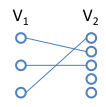
\includegraphics{diagrams/def14_example1.png}
\end{example*}

\begin{definition}
    A directed graph is a pair $G = (V,E)$ where $V$ is a set of nodes (vertices) and $E$ is a set of edges together 
    with a function $i: E -> V x V$. If $i(e) = (v_{1},v_{2})$ then $v_{1}$ is called start point, $v_{2}$ is called end point.
\end{definition}
Graphically: \\[3mm]
If $i(e) = (v_{1},v_{2})$ we draw 1. \\
If $i(e') = (v_{1},v_{2})$ then this indices a second edge (2.). \\
If $i(e_{1}) = i(e_{2})$ we call $e_{1},e_{2}$ parallel. \\
If $i(e) = (v,v)$ then $e$ is called a directed loop. \\
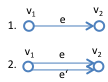
\includegraphics{diagrams/def15_directd_graph.png} \\
$g_{out}(v)$ is the number of edges that have starting point $v$. \\
$g_{in}(v)$ is the number of edges with endpoint $v$.

\begin{lemma}
    $\displaystyle\sum\limits_{v \in V} g_{in}(v) = \displaystyle\sum\limits_{v \in V} g_{out}(v)$
\end{lemma}

\begin{prooof}
    We start with a graph without edges. Then we insert one after the other edges in $E$. 
    Each edge contributes 1 to both sides of the equation.
\end{prooof}

\begin{definition}
    A directed path is a sequence of edges $e_{1},e_{2}...$ such that the end point of $e_{i}$ is the start point of
    $e_{1} +1, i > 1$([NW] +1 seems strange to me, correct?). \\[3mm]

    A directed path $e_{1}...e_{k}$ is called a (directed) \underline{cycle}, if the start point of $e_{1}$ and
    the end point of $e_{k}$ coincide. \\
    A simple (directed) path is a path where every node occurs at most once. \\
    A directed cycle is called simple if every node except for the start and end node occurs at most once.
\end{definition}

\begin{definition}
    A graph directed or undirected is called \underline{simple}, if it does not contain parallel edges.
\end{definition}

\begin{definition}
        A directed graph is called \underline{strongly connected} if for any pair of nodes $(u,v)$ 
        there is a directd path from $u$ to $v$.
\end{definition}

Let $G$ be a directed graph $G = (V,E)$. $x,y \in V x \textasciitilde y$ ([NW] does \textasciitilde mean are "connected"?)
if there is a directed path from x to y and vice versa. \\

The equivalence classes of this relation $~c VxV$ are called strongly connected components.
(Analogously: Define connected components for undirected graphs)

\begin{information}
    We should know how the following terms are defined: reflexivity, symetry, transitivity.
\end{information}

Implementation: \\
1. Adjacency Lists $V = {1...n}, E = {e_{1}...e_{t}}$ \\
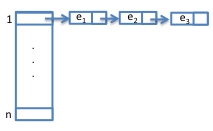
\includegraphics{diagrams/adjacency_list.png} \\
2. Dynamically changing graphs: \\
e.g. multi user databses: Nodes $\equiv$  transactions of user; Edges $\equiv$  waiting situations \\
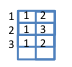
\includegraphics{diagrams/dynamically_changing_graphs.png} \\
Graph is used to detect dead locks. Waiting arises when data are locked by a user that modifies these data. \\
$U_{1}$ $write(d)$, $read(d')$ \\
$U_{2}$ $read(d)$, $write(d')$

\begin{definition}
    An undirected graph is called a tree if it is connected and does not have simple cycles.\\
    Let $G$ be a directed graph, $G=(V,E)$. A node $r$ is called root if every other node can be 
    reached from $r$ via a directed path. \\
    A directed graph is called a tree if it has a root and the underlying undirected graph is a tree. \\
    Let $G$ be a directed graph. A node is called source if $g_{in}(v) = 0$. $v$ is called sink if $g_{out}(v) = 0$
\end{definition}

\begin{lemma}
    NW: what was lemma 1.3? the next one was 1.4 in my notes
\end{lemma}
\begin{lemma}
    If $G=(V,E)$ is a directed graph without directed cycles, then tere is always a source and sink.
\end{lemma}
We use this theorem to detect cycles

\begin{prooof}[Proof: Source (sink analogously)]
    Select an arbitrary node $v_{1}$. If $v_{1}$ is a source we are done. If it is not, then there must be an edge $e_{1}$
    leading to it $v_{2} \xrightarrow{e_{1}} v_{1}$. \\
    If $v_{2}$ is a source we are done. If not, there must be an edge $e_{2}$ leading to it
    $v_{3}  \xrightarrow{e_{2}} v_{2} \xrightarrow{e_{1}} v_{1}$.
    We continue this process. It must stop because there are only finitely many nodes and if a node would appear once more
    on such a path, there would be a directed cycle.
\end{prooof}







\chapter{Euler Graphs and Hamilton Graphs}

\begin{descr}
    TODO
\end{descr}

\section{Euler Graphs}\index{Euler Graphs}
\subsection{Euler 1736: K�nigsberger Br�ckenproblem}
Is it possible to do a round walk crossing every bridge exactly once?\\
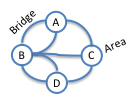
\includegraphics{diagrams/koenigsberg.png}

\begin{example}
    
\includegraphics{diagrams/haus_vom_nikolaus.png}    
\end{example}

\begin{definition}
Let $G$ be a finite undirected graph. A path $e_{1}..e_{t}$ is called a \deftxt{euler path}
if every edge in $E$ occurs exactly once in the list.\\
A graph is a \deftxt{euler graph} if it has a euler path.
\end{definition}

\begin{theorem}
    A finite connected graph is a euler graph if and only if:
    \begin{enumerate}
        \item It has eiter exactly two nodes of odd degree.
        or
        \item All nodes have even degree.
    \end{enumerate}
\end{theorem}

In the last case the path is a cycle. In the first case no euler path is a cycle.
Check is possible in linear time.

\begin{prooof}
    $">"$ Let $G=(V,E)$ be a graph that has a euler path that is not a cycle. Let $\mid E \mid=k$
    $\circ  \xrightarrow{e_{1}} \circ \xrightarrow{e_{2}} ... \circ \xrightarrow{e_{k}}$
    In this path $v_{1}$ and $v_{k+1}$ have odd degreee and all other nodes have even degree. 
    Now consider the case teht $G$ has a euler cycle.\\
    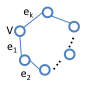
\includegraphics{diagrams/proof21.png} \\
    Hence every node has even degree. \\[2mm]
    
    $"<"$ Let $G$ be a graph with exactly two nodes with odd degree, let this be $a$ and $b$.
    We contradict a euler path as follows:\\
    Start at node $a$ and folow an edge ?inktt? on a. $a\circ  \xrightarrow{} \circ \xrightarrow{} ... \circ b$ \\
    Case 1: All edges have been used -> done \\
    Case 2: Still edges unused. Then because $G$ is connected there must be some node $v$ on 
    the path from which there is an unused edge. We construct a path starting from $v$ as before. This path must end in $v$.\\
    $\Rightarrow$ Repeat until there are no more unused edges.\\
    Analogously we proceed when the degree of all nodes is even.\\
    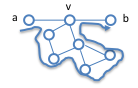
\includegraphics{diagrams/proof212.png} \\
\end{prooof}

\begin{example*}
    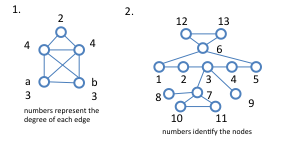
\includegraphics{diagrams/examples21.png} \\ 
\end{example*}

In the directed case a \deftxt{directed Euler path} is a directed path on which every edge appears exactly once.
Directed \deftxt{Euler cycle} analogously.\\

\begin{theorem}
    A finite directed graph is a \deftxt{directed Euler graph} if and only if its underlying undirected graph is connected.
    \begin{enumerate}
       \item There is one node $a$ with $g_{out}(a) = g_{in}(a) + 1$ and another node\\ b with $g_{in}(b) = g_{out}(b) + 1$ and
             for all other nodes $v g_{in}(v) = g_{out}(v)$. Or
       \item For all nodes $g_{in}(v) = g_{out}(v)$ (\deftxt{directed Euler cyle})
             
    \end{enumerate}
\end{theorem}


\section{Hamiltonian Graphs}\index{Hamiltonian Graphs}
\begin{definition}
    Let $G=(V,E)$ be a graph. A \deftxt{Hamiltonian cycle} $C$ is a cycle on which every node $\in V$ occurs exactly once.
    If $G$ has a Hamiltonian cycle it is called  \deftxt{Hamiltonian}.
\end{definition}
\begin{example*}
    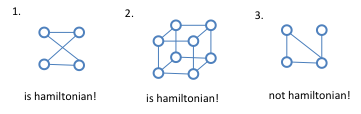
\includegraphics{diagrams/examples22.png} \\ 
\end{example*}


The problem, given an arbitrary undirected graph: Is it \deftxt{Hamiltonian}? $\Rightarrow$ NP complete $\Rightarrow$ no polinomial
time algorithm is known and it is assumed there is no such.\\
One way out of the complexity issue is to derive conditions that can be tested explicitly and if they are satisfied
the desired property is ensured.

\begin{theorem}
    Let $G=(V,E)$ be an undirected finite graph without loops and without parallel edges. Let $\left| V \right|=n$. If for all
    $x,y \in V with x \neq y$ and no edge with end points $x,y$ the following holds: \\
    $deg(x) + deg(v) \geq \left| V \right|=n$ \\
    Then $G$ has a \deftxt{Hamiltonian Cycle}.
\end{theorem}

\begin{example*}
     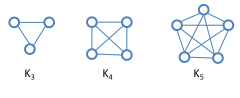
\includegraphics{diagrams/examples23.png} \\ 
\end{example*}
    
\begin{prooof}
    Assume there is a graph $G=(V,E)$ with $deg(x) + deg(y) \geq \left| V \right|$ for all $x$ and $y$ with $x \neq y$
    and no edges between them, but is not \deftxt{Hamiltonian}. Among all graphs with nodes in $V$, we choose one that
    has this property and has the maximal number of edges, we call graph $G_{0}=(V,E_{0})$. As the complete graph
    (every node is connected with every other node) is \deftxt{Hamiltonian}, we know there must be an edge $e$ connecting some $x$ 
    and $y$ and $e \in E_{0}$. \\
    We add edge $e$ to the graph and obtain a new graph $G_{1}=(V,E_{1})$ that still satisfies the degree conditions and must be \deftxt{Hamiltonian}
    because $G_{0}$ was the one with the largest number of edges.\\
    We know that the \deftxt{Hamiltonian cycle} must contain the edge $e$. \\
    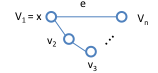
\includegraphics{diagrams/proof23.png} \\ 
    $v_{i} \neq v_{j} for i \neq j$
    
    $S = \{ v_{i}: 1 \leq i \leq n$ x,y are connected with an edge in $E_{0}\}$ \\
    $T = \{ v_{i}: 1 \leq i \leq n $ there is an edge between $y$ and $v_{i}$ in $E_{0}\}$ \\
    
    Observation:
    \begin{enumerate}
        \item $y = v_{n} \in S \cup T$
        \item $\left| S \cup T \right| < \left| V \right| = n$
        \item $deg(x) = \left| S \right|$ \\
              $deg(y) = \left| T \right|$
    \end{enumerate}
    Hence $S \cap T \neq \emptyset, let v_{j} \in S \cap T$ hence there is an edge between $x,v_{j+1}$ and an edge between $y,v_{j}$. Now remove
    edge $e$ and there is a Hamiltonian left. \\
    Cost of checking the condition $O(M^2) \left| E \right| \leq \left| V \right|^2$ \\
    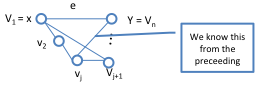
\includegraphics{diagrams/observation23.png} \\ 
\end{prooof}

\section{Bipartite Graphs}\index{Bipartite Graphs}

\begin{example*} 
    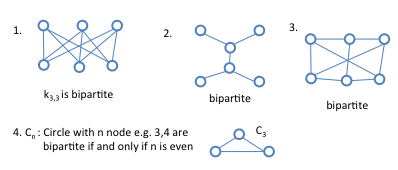
\includegraphics{diagrams/bipartiteexp.png} 
\end{example*}

\begin{theorem}
    Let $G=(V,E)$ be a connected undirected graph without loops and parallel edges. 
    $G$ is bipartite if and only if it does not contain any circle of odd length.
\end{theorem}

Corollary: All trees are bipartite

\begin{prooof}
    $\Rightarrow$ IF $G$ contains a cicle of odd length then it is not bipartite.
    $\Leftarrow$ Let $G$ not have any circle of odd length we choose node v.\\
    $V_{1} = \{ u \in V \text{a shortest path between u and v is of odd length} \}$ \\
    $V_{2} = \{ u \in V \text{a shortest path between u and v is of even length} \}$ \\
    $V \in V_{2}, V = V_{1} \dot{\cup} V_{2}$ (disjoint union) \\
    Claim: Ther is no edge $e$ with both endpoints in $V_{1}$ respectively $V_{2}$. Assume there is an edge $e$ with both
    endpoints in $V_{1}$. Let the end points be $x,y$ \\
    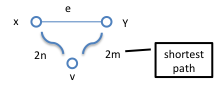
\includegraphics{diagrams/proof24.png} \\
    $2m \leq 2n + 1 \text{and} 2n \leq 2m + 1 \Rightarrow m = n$ \\
    
    Let $P(x)$ a shortest path from $v$ to $x$, analogously $P(y)$ let $w$ be the last node on the paths starting at $v$ that lies
    on both paths.
    
    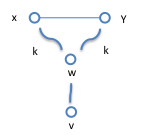
\includegraphics{diagrams/proof242.png} \\
    The length of the path from $w$ to x coincides with the length of path from $w$ to $y$. \\
    The circle w - x - y - w is of odd length i.e. $2k+1 \Rightarrow$ contradiction!
\end{prooof}

Corollary 2.5: A bipartie graph with an odd number of nodes cannot be \deftxt{Hamiltionian}

\begin{prooof}
    Assume if were Hamiltionian then there is a cycle where node appears exactly once. 
    This cycle is of odd length $\Rightarrow$ contradicts Theorem 2.4
\end{prooof}
    
\begin{example}
    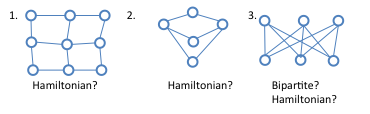
\includegraphics{diagrams/example25.png} \\
    $\Rightarrow$ We have two theorems to check:
    \begin{enumerate}
        \item Count degrees
        \item Corollary 2.5
    \end{enumerate}
\end{example}



\chapter{(Network) Flow Problems}

\begin{descr}
    TODO
\end{descr}

\section{Network Flow Problems}\index{Network Flow Problems}
\begin{example}
Example: Oil field + transportation

\end{example}

\begin{definition}
A network N consists of 
\begin{enumerate}
\item A finite directed graph $G=(V,E)$ without loops and parallel edges
\item a function $c: E -> \mathds{R}^{+}$, which assigns a capacity to each edge
\item two designated nodes s and t, called \deftxt{source} and \deftxt{sink}
\end{enumerate}
Short: $N = (G, c, \{s, t\})$
\end{definition}

\begin{definition}
Let $N = (G, c, \{s, t\})$ be a network. A flow function on N is a function $f: E -> \mathds{R}$ such that 
\begin{itemize}
\item $ 0 \le f(e) \le c(e), \forall e \in E $
\item $ \alpha(v) := \{e:$ endpoint of e is v $\}, v \in V$ \\
$\beta(v) := \{e:$ startpoint of e is v $\}, v \in V$
\end{itemize}
For every $v \in V\backslash\{s, t\} $ \\
$ \sum_{e \in \alpha(v)} f(e) = \sum_{e \in \beta(v)} f(e) $ \\
This is called \deftxt{"conservation function"}. \\
The \deftxt{total flow} of the flow function is given by $F = \sum_{e \in \alpha(t)} f(e) - \sum_{e \in \beta(t)} f(e) $
\end{definition}

\begin{example}
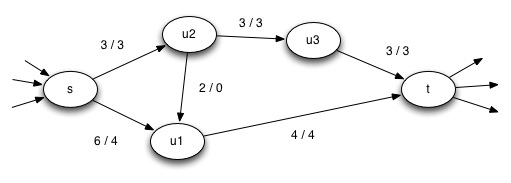
\includegraphics{diagrams/Chapter3_Example1.jpg}
\\Notion: $ 6 / 4 $ describes the capacity and the flow of an edge. In this example the capacity of the edge is 6 and the flow is 4.
\end{example}

Problem: \\
Given an arbitrary network N, find a flow function f, where the total flow F is maximal. \\

\begin{definition}
Let N = $(G, c, \{s, t\})$ be a network. Let $S \subseteq V$ with s $\in S, t \notin S$ \\
$\bar{S} = V \backslash S$ (i.e. $t \in \bar{S}$) \\
$E_{S\bar{S}} = \{e:$ all edges with starting point in S and endpoint in $\bar{S} \}$ \\
$E_{\bar{S}S} = \{e:$ all edges with start point in $\bar{S}$ and end point in S $\}$ \\
$E_{S\bar{S}} \cup E_{\bar{S}S} $ is the \deftxt{cut} defined by S. \\
The capacity of a cut defined by S: $c(S) = \sum_{e \in E_{S\bar{S}}}c(e)$
\end{definition}

\begin{lemma}
Let $N =(G, c, \{s, t\})$ be a network, $f: E \rightarrow \mathds{R}$ be a flow function then for any $S \subseteq V$ with $s \in S, t \notin S$: 
\[
F = \sum_{e \in E_{S\bar{S}}}f(e) - \sum_{e \in E_{\bar{S}S}} f(e)
\]
\end{lemma}

\begin{proof}
\[ F = \sum_{e \in \alpha(t)} f(e) - \sum_{e_ \in \beta(t)} f(e) \]
\[0 = \sum_{e \in \alpha(v)} f(e) - \sum_{e \in \beta(v)} f(e); \forall v \in \bar{S} \backslash \{t\} \]
We add all these equations up. Left hand side: $F$ remains. Right hand side: Let $x \xrightarrow{e} y$ be an edge. We need to consider 4 cases:
\begin{enumerate}
\item $x, y \in S$, then the value $f(e)$ does not occur in the summation
\item $x, y \in \bar{S}$, then $f(e)$ occurs one time positive in the summation, namely for y \\ f(e) occurs one time negative in the summation, namely for x 
\item $x \in S; y \in \bar{S}$, f(e) occurs positive for y and nowhere else and $e \in E_{S\bar{S}}$  \label{xSySbar}
\item $x \in \bar{S}; y \in S$, then $f(e)$ occurs negative for x and nowhere else and $e \in E_{\bar{S}S}$ \label{xSbaryS}
\end{enumerate}
This leads to the following equation:
\[F = \sum_{e \in E_{S\bar{S}}}f(e) - \sum_{e \in E_{\bar{S}S}} f(e) \]
Only case \ref{xSySbar} and \ref{xSbaryS} contribute.
\end{proof}

\begin{lemma}
For every flow function f with total flow F and any ser $S \subseteq V$, $s \in S$, $t \notin S$
$$ F \le c(S) $$
\end{lemma}

\begin{proof}
From lemma 3.1 we know
\[F = \sum_{e \in E_{S\bar{S}}}f(e) - \sum_{e \in E_{\bar{S}S}}f(e) \le \sum_{e \in E_{S\bar{S}}}f(e) \le \sum_{e \in E_{S\bar{S}}}c(e) = c(S) \] 
\end{proof}

\begin{corollary}[Max Flow - Min Cut Statement]
If $F=c(S)$ then the total flow F is \underline{maximal} and the capacity of the cut defined by $S$ is \underline{minimal}.
\end{corollary}

\begin{proof}
Let $F = c(S)$, consider another flow function $f'$ with total flow $F'$.
\begin{enumerate}
\item $F' \le c(S)$ (Lemma 3.2) // $F' \le c(S) = F$ \\Hence, f is a flow function with maximal total flow.
\item Let $S'$ with $s \in S'$, $t \notin S'$ be given. $c(S) = F \le c(S')$. Hence the capacity $c(S)$ is minimal among all other capacities. 
\end{enumerate}
\end{proof}

An \deftxt{augmenting path} is a simple path from s to t, that is not necessarily directed. And for which the following two cases hold: Let e be an edge on this path: 
\begin{enumerate}
\item $ s \rightarrow \circ \rightarrow \circ \rightarrow ... \rightarrow \underset{s_i}{\circ} \xrightarrow{e} \underset{s_{i+1}}{\circ} ...  \underset{t}{\circ}$ then we request that $f(e) < c(e)$
\item $s \rightarrow \circ ...  \underset{s_i}{\circ} \xleftarrow{e} \underset{s_{i+1}}{\circ} ... \underset{t}{\circ}$ then we request that $f(e) > 0$
\end{enumerate}

\begin{example}
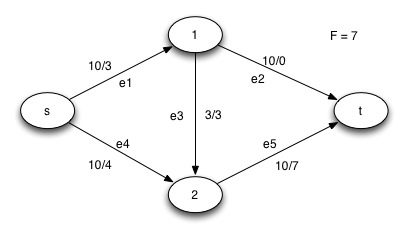
\includegraphics{diagrams/Chapter3_Example2.jpg} \\
Which of the following is an augmenting path? 
\begin{itemize}
\item $e_1 e_2$
\item $e_1 e_3 e_5$
\item $e_4 e_3 e_2$
\item $e_4 e_5$
\end{itemize}

Solution: \\
The first, third and fourth example are augmenting paths. The second path violates case 1.
\end{example}

We use $e_4 e_3 e_2$ to improve the flow function as follows:
\begin{itemize}
\item For forward egdes $e: c(e) - f(e)$:
\begin{itemize}
	\item $e_4: 6$
	\item $e_2: 10$
\end{itemize}
\item For backward edges $e: f(e)$
\begin{itemize}
\item $e_3: 3$
\end{itemize}
\end{itemize}
We chose the minimum from the values and add the value to the flow of forward egdes and substract it from backward egdes. The flows of the edges change as follows:
\begin{itemize}
\item $e_4 = \xfrac{10}{7}$
\item $e_2 = \xfrac{10}{3}$
\item $e_3 = \xfrac{3}{0}$
\end{itemize} 

\begin{example}
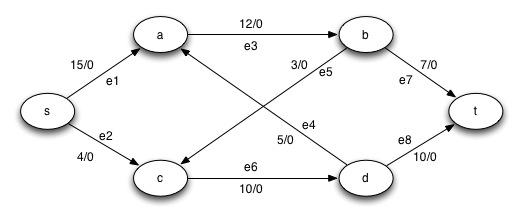
\includegraphics{diagrams/Chapter3_Example3.jpg} \\
Augmenting path: \\
$s* \xrightarrow{e_2} c* \xrightarrow{e_6} d* \xrightarrow{e_4} a* \xrightarrow{e_3} b* \xrightarrow{e_7} t*$ \\
Compute deltas:
\begin{itemize}
\item $\Delta_{(e_2)} = 4$
\item $\Delta_{(e_6)} = 10$
\item $\Delta_{(e_4)} = 5$
\item $\Delta_{(e_3)} = 12$
\item $\Delta_{(e_7)} = 7$
\end{itemize}
The minimum $\Delta$ is 4, so the flow of the edges will be increased by 4.
\begin{itemize}
\item $e_2 = \xfrac{4}{4}$
\item $e_6 = \xfrac{10}{4}$
\item $e_4 = \xfrac{5}{4}$
\item $e_3 = \xfrac{12}{4}$
\item $e_7 = \xfrac{7}{4}$
\end{itemize} 

The next steps or paths would be:
\begin{itemize}
\item $s \rightarrow a \rightarrow b \rightarrow c \rightarrow d \rightarrow t$
\item $s \rightarrow a \rightarrow b \rightarrow t$
\item $s \rightarrow a \rightarrow d \rightarrow t$
\end{itemize}
The application of this paths leads to a new flow: $F = 14$.
\end{example}

\begin{lemma}
When executing a step in the algorithm, the actual function f is a flow function.
\end{lemma}

\begin{proof}
The assumption is obviously true for step 1 because $f \equiv 0$ is a flow function. It is obviously true for steps 2, 3 and 5, too, because f is not modified. \\
Step 4: \\
Let $f$ be a flow function when we enter step 4. We have to show that after performing step 4, the newly calculated function $f$ is still a flow function. \\
Let $f_{old}$ be the function with which we enter step 4 and $f_{new}$ the newly calculated one. $f_{old}$ is a flow function. Hence, 
\[\sum_{e \in \alpha(v)} f_{old}(e) = \sum_{e \in \beta(v)}f_{old}(e); \forall v : v \neq s, v \neq t\]
Let $s \rightarrow v_0 \rightarrow v_1 ... v_{f_{e-1}} \rightarrow v_{f_e} \rightarrow t$ be an augmenting path used in step 4. By definition of $\Delta f_{new}(e) < c(e)$ and $f_{new}(e) > 0$. \\
For step 4: Let $s = v_0 \rightarrow ... \rightarrow v_2 = t$ be the path along which we achieved the marking. Only the flow value of the edges along this path is modified, so we have to check only the edges respectively nodes along this path. We have to check: 
\begin{enumerate}
\item $ 0 \le f_{new}(e) \le c(e) \forall e$: e edge on the path
\item $\sum_{e \in \alpha(v)} f_{new}(e) = \sum_{e \in \beta(v)}f_{new}(e),  \forall v$, v on the path, $v \neq s, v \neg t$ 
\end{enumerate}
The check: 
\begin{enumerate}
\item 1 holds by the definition of $\Delta$
\item Let $v_i, v_i \neq s, v_i \neq t$ be a node on the path:
\begin{enumerate}
\item $\xrightarrow{e_i} v_i \xrightarrow{e_{i+1}}, e_i \in \alpha(v_i), e_{i+1} \in \beta(v_i)$ for both edges $f_{new}$ is obtained from $f_{old}$ by adding $\Delta$, so 2 holds in this case
\item $\xrightarrow{e_i} v_i \xleftarrow{e_{i+1}}, e_i, e_{i+1} \in \alpha(v_i)$. One contributes $\Delta$, the other contributes $-\Delta$, so 2 holds for $v_i$
\item $\leftarrow v_i \leftarrow$ analogously
\item $\leftarrow v_i \rightarrow$ analogously, too
\end{enumerate}
\end{enumerate}
\end{proof}

\begin{lemma}
If the algorithm by Ford-Fulkerson terminates then the determined flow function has maximal total flow.
\end{lemma}

\begin{proof}
If the algorithm terminates, then it does so in step 3. That means we started labeling but did not reach $t$. Let $S$ be the set of nodes that were marked in the last round. Then $s \in S$ and $t \notin S$. $\bar{S} = V \backslash S$. Let $x \xrightarrow{e} y$ be an edge in $E_{S\bar{S}}$, this means x is labelled, y is not labelled. So, we know that $f(e) = c(e)$ because otherwise we could have marked y.\\
If $x \xrightarrow{e} y$ is an edge in $E_{\bar{S}S}$ ($x \in \bar{S}, y \in S$). So, $y$ is labelled and $x$ is not. Then we can conclude that $f(e) = 0$, otherwise we could have marked $e$. 
\[F \stackrel{(3.1)}{=} \sum_{e \in E_{S\bar{S}}}f(e) - \underbrace{ \sum_{e \in E_{\bar{S}S}}f(e)}_{= 0} = \sum_{e \in E_{S\bar{S}}} c(e) = c(e) \]
f is a flow function with maximal total flow. 
\end{proof}

\deftxt{Termination} \\

\begin{lemma}
If $c: E -> \N$ then the algorithm terminates.
\end{lemma}

\begin{proof}
This holds because the algorithm starts with $f \equiv 0$ and the total flow $F$ is increased by $\Delta$ and $\Delta$ is a natural number as $c(e) \in \N \forall e$ and because $F \le c(s)$ for all $S$ with $s \in S, t \notin S$ i.e. F is bordered. \\
What about $c: E -> \R$? 
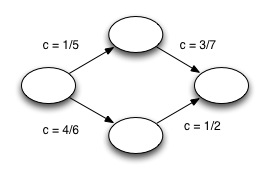
\includegraphics{diagrams/Chapter3_Proof_3_6.jpg} \\
Turn the capacities into natural numbers, calculate the results and divide them later.
\end{proof}

\begin{proposition}
The example with $c: E -> \R \backslash \Q$ is an example, for which we can apply the algorithm in a way that is does not terminate. 
\end{proposition}

\begin{example}
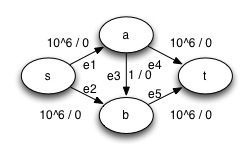
\includegraphics{diagrams/Chapter3_Example_4.jpg} \\
Maximal total flow: $2 * 10^6$ \\
Selecting the augmenthing paths: 
\begin{itemize}
\item $e_1 e_4$ 
\item $e_2 e_5$
\end{itemize}
This would solve the problem within two steps, but... \\
Choosing the following augmenting paths: 
\begin{itemize}
\item $e_1 e_3 e_5$ with $\Delta = 1$ and
\item $e_2 e_3 e_4$ with $\Delta = 1$ 
\end{itemize}
would lead to $2*10^6$ rounds to solve the problem. 
\end{example}

\begin{theorem}
If we use breadth-first-search when labelling and always select the shortest augmenting pathe, then the algorithm terminates and uses $O(|V|^3 * |E|)$ steps for any $c:E -> \R$ (where it is assumed that any real number can be manipulated in one step).
\end{theorem}

\begin{definition}
Let e be an edge between u and v with flow value $f(e)$. e is called \deftxt{useful} from u to v if 
\begin{enumerate}
\item $ u \xrightarrow{e} v$ and $f(e) < c(e)$
\item $u \leftarrow v$ and $f(e) > 0 $
\end{enumerate}
Let $G = (V,E)$ be the directed graph for the network and $f$ a flow function for the network. A \deftxt{layering} for the network is defined as follows: 
\begin{enumerate}
\item $V_0 = \{s\}, i \leftarrow 0$
\item $ T := \{ v \in V, v \notin V_j, j \le i$ and there is an useful edge from a node in V to v $\}$
\item If $ T = \emptyset$ then the actual flow function has maximal total flow and the algorithm stops. 
\item If $t \in T$ then put $l := i+1, V_l = \{t\}$ and stop the algorithm.
\item $V_{i+1} := T, i \leftarrow i+1$ and go to step 2
\end{enumerate}
$E(i) = \{e$: e is an useful edge between some node in $V_{n-1}$ and $V_i \}$
\end{definition}

\begin{example}
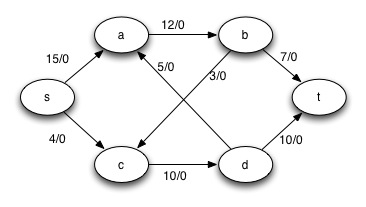
\includegraphics{diagrams/Chapter3_Example5.jpg} \\
Layers:
\begin{itemize}
\item $V_0 = \{s\}$
\item $V_1 = \{a, c \}$
\item $V_2 = \{b, d \}$
\item $V_3 = \{t \}$
\end{itemize}
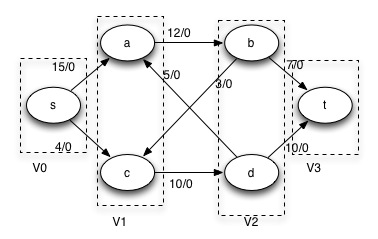
\includegraphics{diagrams/Chapter3_Example5_Solution.jpg} \\
\end{example}

\begin{theorem}
When the algorithm for layering stops in step 3, then the actual flow function has maximal total flow.
\end{theorem}

\begin{proof}
Determine a set S with $F = c(S)$. What S? \\
$ S = \bigcup_{i=0}^i V_j$, $\bar{S} = V \backslash S, s \in S, t \notin S$ \\ 
For any edge $ u \xrightarrow{e} v$, $e \in E_{S\bar{S}}$, we know $f(e) = c(e)$ because otherwise T would not be $\emptyset$. And for any edge $u \xleftarrow{e} v \in E_{\bar{S}S}$ we know $f(e) = 0$ and continue as for lemma 3.5.
\end{proof}

\begin{definition}
Associate capacities $\bar{c}$ to the edges in $E(i)$. Let c be an edge in $E(i)$, $ u \xrightarrow{e} v$ 
\begin{enumerate}
\item if $ u \in V_{i-1}, v \in V_i$, then $\bar{c}(e) := c(e) - f(e)$
\item $u \in V_{i-1}, v \in V_i, u \xleftarrow{e} v$, then $\bar{c}(e) = f(e)$
\end{enumerate}
Remark: \\
$c(e) > 0 $ in both cases as only useful edges are considered in $E(i)$ \\ \\

In the new network we look for a flow function $\bar{f}$ such that on \underline{any} path from s to t 
\[s - v_1 - v_2 - ... - t, v_j \in V_j, e_j \in E_j\]
there is at least one edge e with $\bar{f}(e) = c(e)$. \\
Given such a function $\bar{f}$ (see handout: Denic's algorithm) we modify the original flow function $f_{old}$ as follows:
\begin{enumerate}
\item if $u \xrightarrow{e} v$ with $u \in V_{i-1}, v \in V_i$ then $f_{new}(e) := f_{old}(e) + \bar{f}(e)$
\item if $u \xleftarrow{e} v$ with $u \in V_{i-1}, v \in V_i$ then $f_{new}(e) := f_{old}(e) - \bar{f}(e) $
\end{enumerate}
\underline{Algorithm of Denic:} \\
\begin{enumerate}
\item Initialize with a flow function f, e.g. $f(e) \equiv 0 \forall e \in E$
\item Construct a layering with respect of f (remember: halt twice)
\item Determine $\bar{f}$
\item From f and $\bar{f}$ determine the new flow function
\item Go to step 2
\end{enumerate}
\end{definition}

\begin{example}
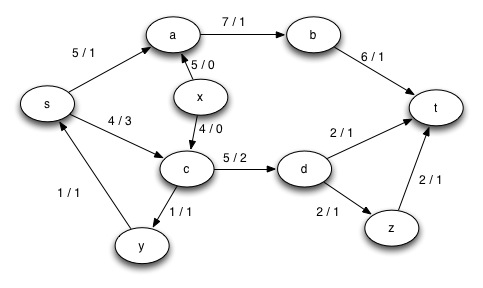
\includegraphics{diagrams/Chapter3_Example6_V1.jpg} \\
Given the example above the total flow of the network is $F=3$. We will proceed with the first layering as follows: \\
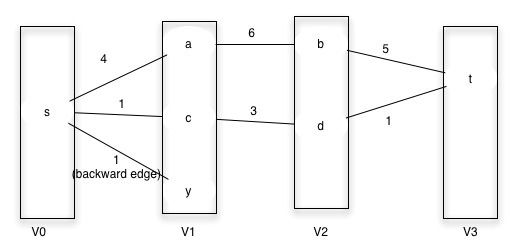
\includegraphics{diagrams/Chapter3_Example_6_Layering1.jpg} \\ 
The nodes $x, z$ disappeared while layering. \\
Determine $\bar{f}$: there are two paths from s to t, find $\bar{f}$ for each of them that saturates at least one edge on the path. The lower path yields a flow function that transports one unit from s to t. The upper path yields a flow function that transports four units from s to t. \\
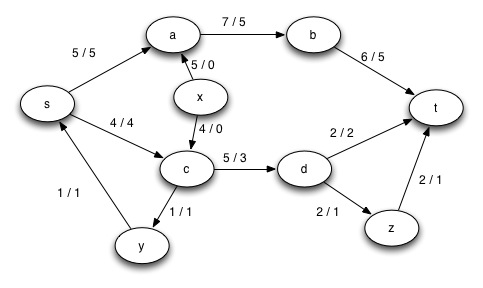
\includegraphics{diagrams/Chapter3_Example6_V2.jpg} \\
After determining $\bar{f}$ we have to update the flows on our graph and gain a new total flow $F=8$. \\
\underline{Second layering:} \\
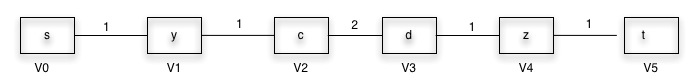
\includegraphics{diagrams/Chapter3_Example_6_Layering2.jpg} \\ 
There is only one path from s to t. A flow function $\bar{f}$ that saturates at least one edge is the one that sends one unit along this path. \\
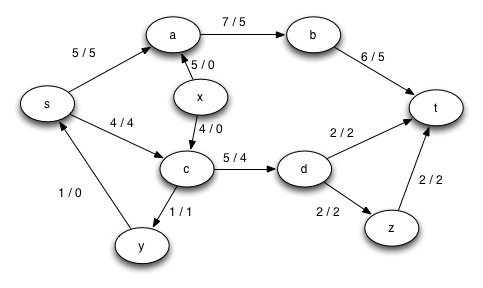
\includegraphics{diagrams/Chapter3_Example6_V3.jpg} \\
We update again the flows of the used edges and the total flow increases by one, so we have: $F=9$. \\
\underline{Third layering} \\
$V_0 = \{s\}$ can not be continued as there are no more useful edges from $V_0$.
\end{example}

\begin{lemma}
Let N be a network with flow function f. $\bar{f}$ is the flow function of the layered network. Then 
\begin{enumerate}
\item the new calculated function f is a flow function and
\item the new total flow is obtained by adding the old total flow and $\bar{F}$($F_{old} + \bar{F} = F_{new}$).
\end{lemma}
% ================================

\ifthenelse{\equal{\useThumbs}{1}}
	{\ihead[]{}}{}
\ifthenelse{\equal{\useIndex}{1}}{
\clearpage
\renewcommand{\indexname}{Index}
\printindex}{}
\end{document}